\title{Numerical Statistical Mechanics}
\author{
        Kevin Belleville \\
        University of California, Los Angeles\\
        Physics 188B, Josh Samani\\
}
\date{\today}

\documentclass[12pt]{article}

\usepackage{braket}
\usepackage[margin=1in]{geometry}
\usepackage{graphicx}
\usepackage{float}

\begin{document}
\maketitle

\begin{abstract}
We learn about the Metropolis-Hastings algorithm and apply it to an Ising model to model magnetic dipoles and their interactions with each other as we vary temperature.
\end{abstract}

\section{Introduction}

\subsection*{The Metropolis-Hastings Algorithm}

The Metropolis algorithm is a Markov chain Monte Carlo simulation. In short, a Monte Carlo simulation takes repeated random sampling to numerically compute solutions; and a Markov chain is a way to compute probabilities randomly. A Markov chain is basically: if you are in a certain state, you have a certain probability of staying at that state, or changing to a different state. The Metropolis algorithm takes advantage of this by using a Markov chain to create a probability distribution. 

\subsection*{The Ising Model}

The Ising model is a model of magnetic dipole moments; in our case, we use a 2D array. Every point in the array is either spin up or spin down, and we use the Metropolis algorithm to compute the change in the array. There is a certain probability that the point will switch spin or stay at the same spin, depending on its neighbors to its top, bottom, left, and right sides. In our case, we use the model to show a phase transition between the states of magnetism. This model can also be extrapolated to involve a external magnetic force, but we simplify our case to have none. To elaborate on the method we use to change the model over time, we calculate the change in energy with a certain point's neighbors -- if the energy change is less than zero, we immediately accept the new state. This is because nature is always trying to find a state of equilibrium, where the energy is the lowest. (Although, one should not think of nature has "trying to find" the "best" state.) Otherwise, if the energy is greater than the current state, we accept it with a certain probability:

\begin{equation}
A = e^{-\Delta E / T}
\end{equation}

We iterate this algorithm many times until the model reaches sufficient equilibrium. Below are figures depicting the Ising models for different temperature ranges. It should be noted that each of these diagrams began with a different randomly generated array -- thus, the large patches will be different rather than similar if one had used the same array.

\begin{figure}[H]
\begin{center}
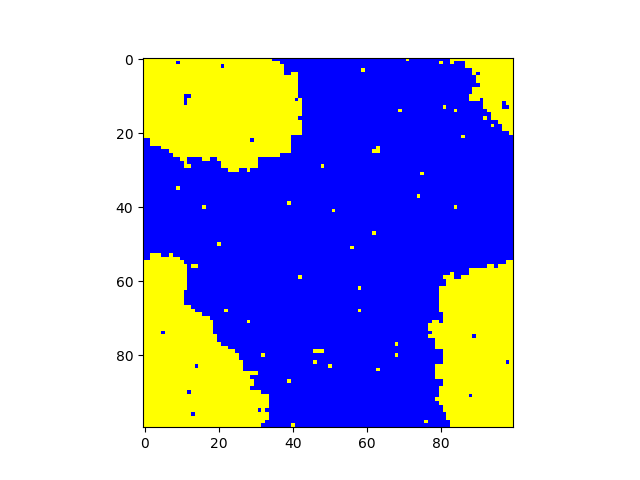
\includegraphics[scale=0.6]{low_temp.png}
\caption{Ising model, 1000 repitions, Temperature = 1.5 (Low)}
\end{center}
\end{figure}

\begin{figure}[H]
\begin{center}
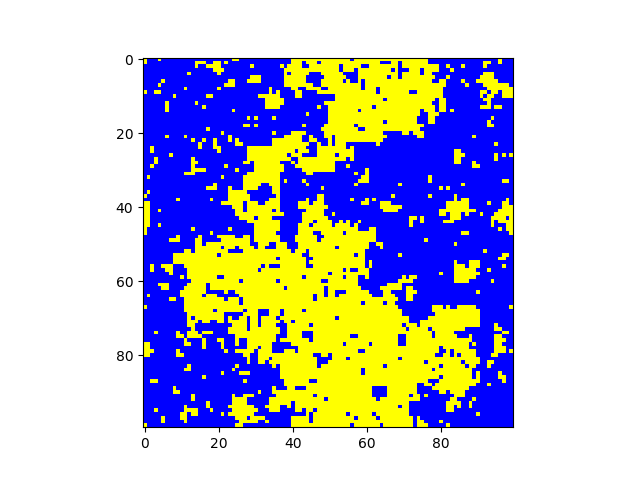
\includegraphics[scale=0.6]{crit_temp.png}
\caption{Ising model, 1000 repitions, Temperature = 2.26 (Critical)}
\end{center}
\end{figure}

\begin{figure}[H]
\begin{center}
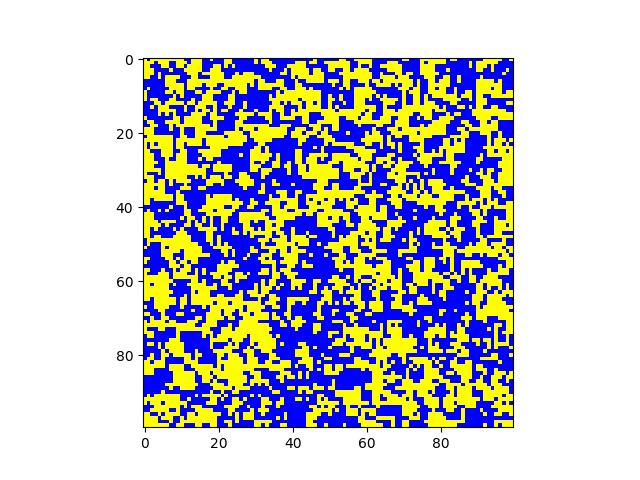
\includegraphics[scale=0.6]{high_temp.png}
\caption{Ising model, 1000 repitions, Temperature = 3.5 (High)}
\end{center}
\end{figure}

Analyzing these diagrams, one can notice that the discord in the higher temperatures is obvious, whereas in the low temp, the patches are much larger and more pronounced. This makes sense when one thinks about the Metropolis algorithm used in equalizing these plots. The temperature in the "random" part of the probabilty $A$ is the only part that the temperature is used in the calculation. If the temperature were much lower, the probability would also be much lower. This would cause the chance of a acceptance happening outside of the energy state being lower than zero to be near zero. Thus larger patches will become apparent. The opposite happens for when temperatures are higher. The random probability will be much higher, causing more discord. This discord will also change the energy states much faster, allowing the patches to "decay", essentially. The critical temperature graph is a compromise between the two.


Side note: there was a very cool website I found that performed many more steps than I could, and allowed for adjustable temperatures on the fly. It was very cool, and I included it in my bibliography. An interesting thing I noted, is that when the temperature was set to the lowest point (0.01), the patches began to try to "overtake" one another, and smaller bubbles of one spin would be "killed". It reminded me a lot of Conway's Game of Life, but the Ising model and the Metropolis algorithm just felt like a much more interesting idea. The projects are similar, but not the same.

\section{Assignment}

\subsection*{Various Quantities vs. Temperature}

\begin{figure}[H]
\begin{center}
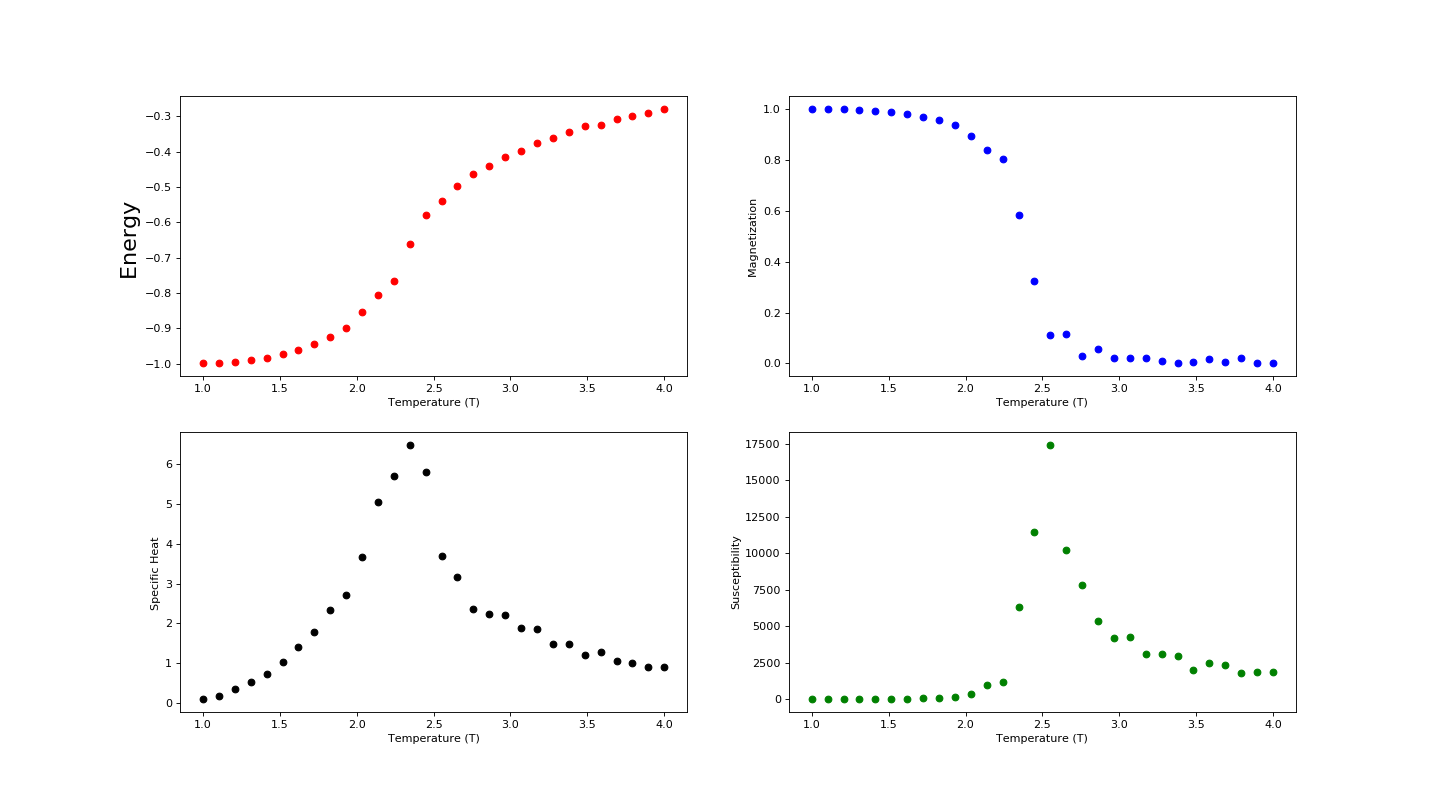
\includegraphics[width=\textwidth]{quants.png}
\end{center}
\end{figure}

The figure above shows all four different quantities, Energy, Magnetism, Specific Heat, and Magnetic Suspectibility. One thing to note is that the code that produced this did this on a 20 x 20 grid rather than a 100 x 100 grid like in the graphs above. A specific point we must be wary of is the critical temperature, defined as:

\begin{equation}
T_c = \frac{2}{\log \left( 1+\sqrt{2} \right) } \approx 2.2692
\end{equation}

We can see that the Energy gradually increases, and begins to slow down once it hits the critical temperature. On the contrary, magnetism starts high, and suddenly decreases to zero once it reaches the critical temperature. Further information about this is provided in the next section, comparing it to an exact solution. The specific heat spikes at the critical temperature. The same happens for the suspectibility but there is no gradual increase from the lower temperature side.


\subsection*{Magnetization: Numerical vs. Onsager's Exact Solution}

\begin{figure}[H]
\begin{center}
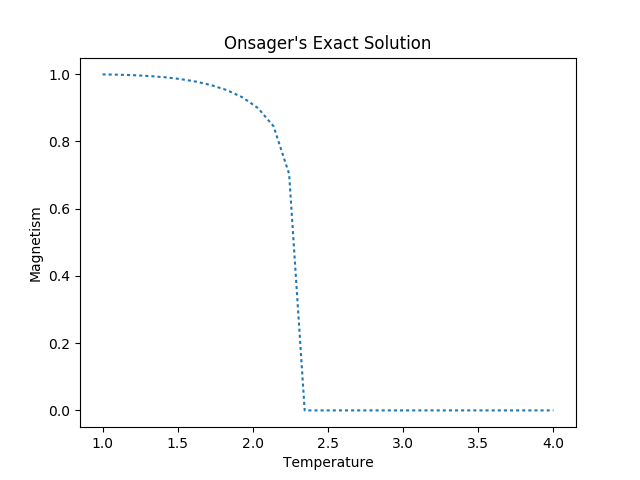
\includegraphics[scale=0.8]{onsager.png}
\end{center}
\end{figure}

Comparing this exact solution to the numerical solution in the section before this, we can see that the numerical solution does follow the exact solution. We can also see that there is actually some variation near the critical temperature's spot in the numerical solution. This is interesting because it is due to the parameters I set in the code. If my code could handle much higher amounts of computations and more precise time points, we would see this error go away.



\section{Conclusions}

This project taught me things relating to Physics as well as coding (which is what this class is all about really). Analyzing a Ising model in such great detail gives me a much deeper understanding about the real world. Similuating a 100 x 100 grid also turned out to be much more difficult than I thought it would be; And simply thinking about how a magnet would have millions upon millions of these interactions is abolutely mind-blowing. I made the same realization in my last project, but this one only reinforces that idea. Also the idea of phase transitions as anything other than solid, liquid, gas, or plasma was unknown to me, which is a little embarrassing for a Physics major.


The coding portion of the project taught me about two different things. One is implementing large-scale arrays and gathering data from them. Python is not the best language for anything like this, as it is very slow in these long computations and I am genuinely mildly confused about why Python would be used. Other languages like C or functional languages I hear are much faster, yet Python is on the rise. I wonder if this is because Python is an easy scripting langauge to get into that allows the programmer to focus more on the ideas of the code rather than the syntax and algorithms. Nevertheless, I still love Python.


Anyway, I also loved learning about the Markov chains, and the Metropolis algorithm. I had heard of Markov chains before, but the only interesting things I had seen come of it were the bots writing random sentences from data scraping the web. Although that was very interesting, the Metropolis algorithm is a very practical implementation of it. This is definitely an algorithm that I will be keeping in my back pocket algorithm handbook for later use in future projects. Some ideas I have been thinking about are extrapolating this algorithm to more than just the spins -1 and 1, to more possible values -- maybe creating a heat map for different things such has population densities, or any other kind of data.



\begin{thebibliography}{9}

\bibitem{a} Weber State University, Daniel V. Schroeder,
\\\texttt{http://physics.weber.edu/schroeder/software/demos/IsingModel.html}

\bibitem{b} Big Theta,
\\\texttt{http://bigtheta.io/2016/02/29/the-ising-model.html}

\bibitem{d} MIT,
\\\texttt{http://web.mit.edu/krish\_s/www/files/ising\_Model.pdf}

\bibitem{e} 
red-starter on GitHub, 
\\\texttt{https://github.com/red-starter/Ising-Model/blob/master/Ising\_model.py}



\end{thebibliography}

\end{document}
